
\documentclass[12pt]{article}
\usepackage[margin=1in]{geometry}
\usepackage{graphicx}
\usepackage{listings}
\usepackage{amsmath}
\usepackage{hyperref}
\usepackage{titlesec}
\usepackage{float}
\usepackage{longtable}
\usepackage{caption}
\titleformat{\section}[block]{\Large\bfseries}{\thesection}{1em}{}
\title{Lab Report: Deploying TFLite \& ONNX Models on Raspberry Pi}
\author{Enugu Harish Reddy \\ 12503787 \\ Embedded Systems \\ Instructor: Prof. Tobias Schaffer}
\date{24-06-2025}

\begin{document}

\maketitle

\section*{1 Introduction}
The main aim of this lab is to evaluate the performance of two pre-trained machine learning models deployed in TensorFlow Lite(TFLite) and ONNX formats on a Raspberry pi by creating a virtual Python environment on a resource constrained edge device. The main relevance of this lab is in the fields of edge computing and Internet of Things(IOT) where deploying efficient AI models on small, low-power devices like Raspberry pi, Arduino boards, Drones and Smart sensors, etc is critical and this also help in understanding how different format models behave on those devices and choosing the right strategy for real-time applications.



\section*{2 Methodology}
 The pre-trained models namely ‘model.tflite’ and ‘model.onnx’ were deployed on a Raspberry Pi using Python and windows power shell using the \textbf{scp} command. We ran both the models in a Virtual Python environment on the Raspberry pi and compared their runtime for evaluating their efficiency . Dummy input data matching the model's expected shape was generated, and inference was performed using Python scripts. Execution time was measured to compare the performance of both model formats.


\subsection*{2.1 Hardware/Device Used}
\begin{itemize}
\item Raspberry Pi 4 Model B, ARM Cortex-A72 CPU, 4GB RAM
\item Used as the edge device to run pre-trained ML models in TFLite and ONNX format.
\end{itemize}

\subsection*{2.2 Programming Language}
\begin{itemize}
\item Python 3 with TensorFlow and ONNX Runtime support
\end{itemize}

\subsection*{2.3 Development Environment}
\begin{itemize}
\item  · Raspberry Pi OS (Linux-based) terminal environment
\item Scripts written using Nano or Vim text editors directly on the Pi
\item SSH used for remote access
\item Virtual environment (venv) used to manage Python packages

\end{itemize}

\subsection*{2.4 Libraries/Frameworks Used}
\begin{itemize}
\item \textbf{TensorFlow}: For running .tflite models using tf.lite.Interpreter()

\item \textbf{ONNXRuntime}: For executing .onnx models using InferenceSession()

\item \textbf{NumPy}: For creating dummy input arrays matching the model’s input shape

\item \textbf{Time}: For measuring inference runtime in seconds

\end{itemize}

\subsection*{2.5 Algorithm Steps}

\begin{enumerate}

\item  Set up and activate a Python virtual environment on the Raspberry Pi

\item  Install required libraries: tensorflow, onnxruntime, and numpy

\item  Transfer model.tflite and model.onnx to Raspberry Pi using scp


\item  Write and run run\_tflite.py to:
  \begin{itemize}
  \item Load the TFLite model 
  \item Allocate tensors and prepare dummy input
 \item  Run inference and print output + inference time
  
\end{itemize}
\item Load the TFLite model 
  \begin{itemize}
 \item	Load the ONNX model
 \item	Prepare dummy input
 \item inference and log output + inference time
  \end{itemize}


6. Compare the performance of both models based on speed and output.

\end{enumerate}

\subsection*{2.6 Data Structures Used}
\begin{itemize}
\item numpy.ndarray: For holding dummy input data

 \item  float: Used for storing and printing inference time

 \item dict and list structures: To access input/output tensor information from models

\end{itemize}

\subsection*{2.7 Tools Used}
\begin{itemize}
\item Raspberry Pi 4 Model B

\item SSH (for remote access and file transfer)

\item \textbf{scp} (for secure file transfer from local machine to Pi)

\item Python Virtual Environment (venv)

\item Terminal for running scripts and viewing output

\end{itemize}

\subsection*{2.8 File and Code Organization}
\begin{itemize}
\item model.tflite – Pre-trained TFLite model
\item model.onnx – Pre-trained ONNX model
\item run\_tflite.py – Python script to run TFLite inference
\item run\_onnx.py – Python script to run ONNX inference
\item All files stored in the home directory of the Raspberry Pi for simplicity

\end{itemize}

\subsection*{2.9 Software and Hardware Used}
\begin{itemize}

\item \textbf{Programming Language}: Python 3

 \item \textbf{Libraries}: NumPy, TensorFlow, ONNX Runtime

 \item  \textbf{Hardware}: Raspberry Pi (CPU execution only, no GPU)

\end{itemize}

\section*{2.10 Code Repository}
Since I have not published this code on Github, I would like to present the code here itself 

 The code includes:

 1. TFlite Inference Script

2. ONNX Inference Script


\subsection*{TFLite Inference Script}
The code for generating a TFLite model ands train it using dummy values is depicted below:- 

\begin{table}[H]
\centering
\begin{tabular}{|p{1\textwidth}|}
\hline
\begin{minipage}{\linewidth}
\begin{lstlisting}[language=Python]
import numpy as np
import tensorflow as tf
import time

interpreter = tf.lite.Interpreter(model_path="model.tflite")
interpreter.allocate_tensors()
input_details = interpreter.get_input_details()
output_details = interpreter.get_output_details()

input_shape = input_details[0]['shape']
dummy_input = np.random.rand(*input_shape).astype(np.float32)

start = time.time()
interpreter.set_tensor(input_details[0]['index'], dummy_input)
interpreter.invoke()
output = interpreter.get_tensor(output_details[0]['index'])
end = time.time()

print("TFLite predicted class:", np.argmax(output))
print(f"TFLite inference time: {end - start:.6f} seconds")
\end{lstlisting}
\end{minipage}
\\ \hline
\end{tabular}
\caption{TFLite inference script inside a table}
\end{table}


\subsection*{ONNX Inference Script}
The code for generating a ONNX runtime format model that is to be deployed to raspberry pi is :-

\begin{table}[H]
\centering
\begin{tabular}{|p{1\textwidth}|}
\hline
\begin{minipage}{\linewidth}
\begin{lstlisting}[language=Python]
import numpy as np
import onnxruntime as ort
import time

session = ort.InferenceSession
("model.onnx", providers=['CPUExecutionProvider'])
input_name = session.get_inputs()[0].name
input_shape = session.get_inputs()[0].shape

dummy_input = np.random.rand(*input_shape).astype(np.float32)
start = time.time()
output = session.run(None, {input_name: dummy_input})
end = time.time()

print("ONNX predicted class:", np.argmax(output[0]))
print(f"ONNX inference time: {end - start:.6f} seconds")
\end{lstlisting}
\end{minipage}
\\ \hline
\end{tabular}
\caption{ONNX inference script inside a table}
\end{table}


\section*{2.11 Code Implementation}
The below pictures(screen shorts) depicts the Implementation of codes in a virtual Python environment(version 3) using Pre-trained Models. A virtual enivironment is created and the models were run using dummy inputs to get an output. Some random snapshots were taken to represent the implementation of the code and are presented below.


\begin{figure}[H]
\centering
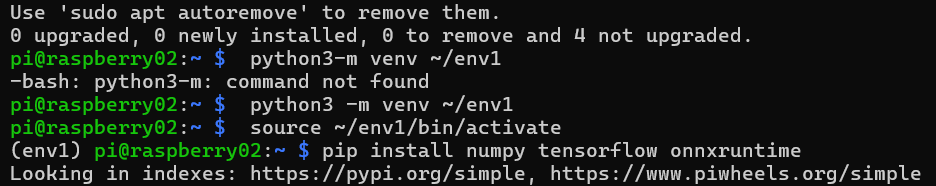
\includegraphics[width=1\textwidth]{screenshot1.png}
\caption{The picture shows the creation of  a virtual python environment to run the models  }
\end{figure}

\begin{figure}[H]
\centering
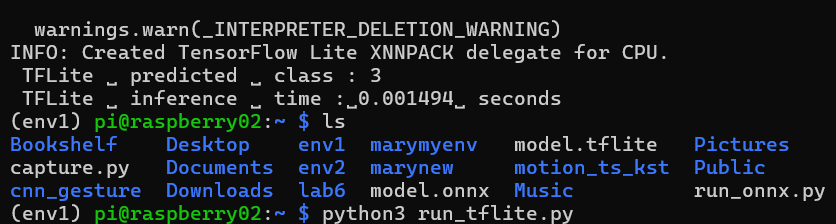
\includegraphics[width=1\textwidth]{screenshot2.png}
\caption{Model files on Raspberry Pi}
\end{figure}

\section*{3 Results}
After deploying the TFLite and ONNX models on the Raspberry Pi, each model was run twice using randomly generated dummy input data. The predicted classes and inference times for each run were recorded and are summarized in the table below.

The variations in predicted class are expected due to the use of random input on each run. All inferences were executed on CPU-only, without any hardware acceleration.






    \subsection*{3.1 TFLite Inference Script}
    The results obtained while running the tensor flow model are:-


    
\begin{figure}[H]
    \centering
    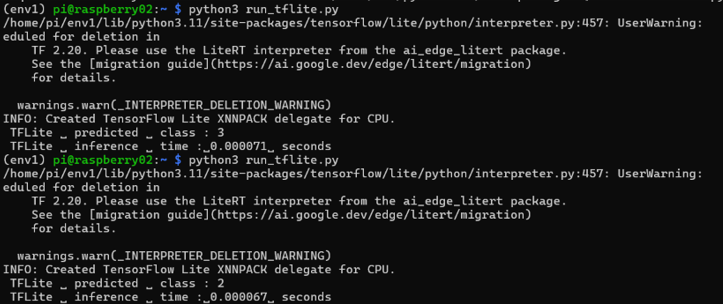
\includegraphics[width=1\linewidth]{Screenshot3.png}
    \label{fig:enter-label}
\end{figure}

 
\subsection *{3.2 ONNX Inference Script}

The results obtained while running the ONNX model in the virtual python environment are :-


\begin{figure}[H]
    \centering
    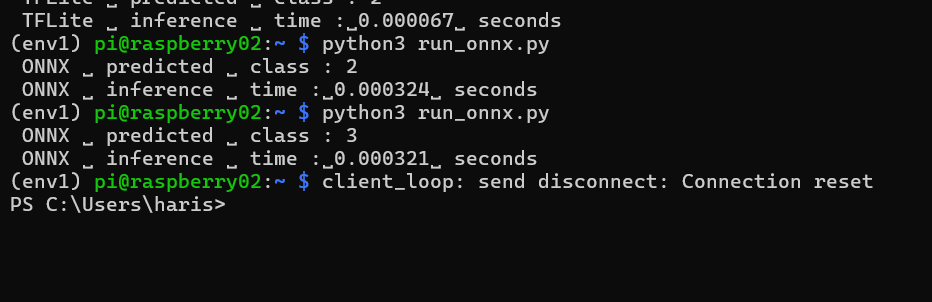
\includegraphics[width=1\linewidth]{Screenshot4.png}
    \label{fig:enter-label}
\end{figure}


\section*{4 FINAL OUTPUT} 

The following table classifies the outputs and identifies the efficient model in the 

experiment 

From the table, We can clearly identify that TFLite model was more efficient than ONNX model according the results of the run values 

\begin{longtable}{|c|c|c|c|c|}
\hline
Run & Format & Predicted Class & Inference Time (s) & Library Used \\
\hline
1 & TFLite & 2 & 0.000067 & TensorFlow Lite \\
2 & TFLite & 2 & 0.000070 & TensorFlow Lite \\
3 & ONNX & 2 & 0.000324 & ONNX Runtime \\
4 & ONNX & 3 & 0.000321 & ONNX Runtime \\
\hline
\end{longtable}


\section* {4  Challenges, Limitations, and Error Analysis}

 During the implementation and testing of the deployment of TFLite and ONNX models on the Raspberry Pi, several challenges were encountered, along with some minor errors and limitations. These aspects are important to reflect on, as they affect the repeatability, scalability, and overall usability of machine learning on edge devices.

\subsection*{4.1 Challenges Faced}

 · Deploying two different format pre-trained models into the raspberry pi

· Ensuring compatibility between model input shapes and dummy data

· Installing ONNXRuntime properly on Raspberry Pi with ARM architecture

\end{itemize}
\subsection*{ 4.2 Error Analysis}
\begin{itemize}

\item Minor syntax mismatches while indexing tensors (['index'])

\item  Connection dropped unexpectedly during SSH session due (client\_loop: send disconnect)

\item The variation in predicted classes across runs is due to the use of randomized dummy input data, which naturally produces different outputs for each inference.

\end{itemize}
\subsection*{4.3 Limitations}
\begin{itemize}

\item Only CPU inference tested; no GPU acceleration

\item Models tested with dummy inputs, not real-world data, so the results only reflect performance, not actual model accuracy or reliability in practical applications.

\item Power consumption, heat generation, and thermal throttling were not measured, though they are important in edge deployment scenarios.
\end{itemize}

\section*{5 Discussion}
The lab results from the experiment support that the common observation that TFLite is better suited for lightweight, real-time applications on edge devices, while ONNX serves well in more flexible, cross-platform environments. The use of dummy inputs ensured safe testing, although it limits accuracy evaluation as the real-time values may affect the performance 

This lab highlighted practical issues such as dependency compatibility, network transfer errors, and the importance of understanding input/output tensor handling, all of which are crucial in real-world embedded ML deployment 

\section*{6 Conclusion}
 This lab successfully demonstrated how to deploy and run both TFLite and ONNX models on Raspberry Pi. TFLite showed better performance, reinforcing its suitability for mobile and embedded systems. Future work could explore real-world input data and GPU/accelerator compatibility.

Future improvements could include testing with real input data, adding more model types for comparison, enabling hardware acceleration, and monitoring power and thermal metrics for a more complete performance analysis.


\end{document}
